%! TEX program = xelatex
%% Filename: sample.tex
%% 
\documentclass[twoside, UTF8, phd, AutoFakeBold]{nputhesis}

\usepackage{lipsum}

%%%%%%%%%%%%%%%%%%%%%%%%%%        biblatex     %%%%%%%%%%%%%%%%%%%%%%%%%%%%%%
% 使用 biblatex 处理参考文献, 格式使用 gb7714-2015
% https://github.com/hushidong/biblatex-gb7714-2015
% 该宏包已包含在 TeXLive 和 MikTeX 中.
% gbnamefmt 参数需要 v1.0k 版本. 如果出错, 可以注释掉第15行.
\usepackage[backend=biber,
            style=gb7714-2015, maxbibnames=3,minbibnames=3,
            gbnamefmt=givenahead,
            doi=false,
            url=false,
%            gbpub=false
           ]{biblatex}

\addbibresource{ref.bib}        % 添加参考文献文件, 必须加后缀.
%%%%%%%%%%%%%%%%%%%%%%%%%%        biblatex     %%%%%%%%%%%%%%%%%%%%%%%%%%%%%%

% \usepackage[super,square,colon,sort&compress]{natbib}

\theoremstyle{npuplain}
\newtheorem{theorem}{定理}[section]
\newtheorem{lemma}[theorem]{引理}
\newtheorem{remark}[theorem]{注}
\newtheorem{definition}[theorem]{定义}
\newtheorem{example}{例}[section]
\newtheorem{assumption}{假设}
\renewenvironment{proof}[1][]{{\noindent\bf\emph{#1证明}: }}{\hfill $\Box$ \\}

\theoremstyle{nputheorem}
\newtheorem{npu-thm}{斜体定理}[section]

\schoolno{10699}
\classno{O.242}
\secretlevel{公开}
\authorno{0000999999}

\title[\LaTeX\ Template of NPU Thesis]{西工大硕博学位论文 \LaTeX 模板}

\author[San Zhang]{张\,\,三}
\major[Philosophy in Mathematics]{数学}
\supervisor[Si Li]{李四}
\applydate[April 2046]{2046~年~4~月}
\support{本文研究得到某某基金(编号:XXXXXXX)资助。}

\begin{document}
\makecover    % 生成中英文封面.

\frontmatter  % 分割封面与前言部分.

% 中文摘要
\begin{abstract}
  \LaTeX 是一种基于 \TeX 的排版系统, 它非常适用于生成高印刷质量的科技和数学,化
  学类文档. \LaTeX 把排版的细节隐藏在若干样式之后, 以内容的逻辑结构统帅复杂的格
  式, 现已成为科技文写作特别是数学写作的重要工具之一. 然而 NPU 仅提供了博士论文
  的 Word 模板. 鉴于此, 我们根据官方 Word 模板制作该模板, 以满足使用 \LaTeX 写
  作论文的需求.

  本模板基本实现了官方格式要求: 封皮, 页眉页脚, 章节标题格式, 参考文献格式等.

  \lipsum[1-5]
  \begin{keywords}
    学位论文, \LaTeX\ 模板, 西工大
  \end{keywords}
\end{abstract}

% 英文摘要
\begin{Abstract}
  \lipsum[1-4]
  \begin{Keywords}
    Thesis Template, \LaTeX, NPU
  \end{Keywords}
\end{Abstract}

\tableofcontents    % 目录
\printnomenclature  % 符号命名表 添加符号可用 
                    % \nomenclature{<sym>}{<text explanation>}

\mainmatter         % 分割目录和正文部分

% 添加符号  这些可在正文中任意的地方
\nomenclature{$\mathbb{R}^n$}{$n$ 维欧几里得空间}
\nomenclature{$\Omega$}{空间 $\mathbb{R}^n$ 中的开集}
\nomenclature{$L^p(\Omega)$}{Lebesgue 空间}
\nomenclature{$W^{m,p}(\Omega)$}{Sobolev 空间}
\nomenclature{$H^m(\Omega)$}{具有 $m$ 阶 $L^2$ 导数 的 Sobolev 空间}
\nomenclature{$C^k(\Omega)$}{具有 $k$ 阶连续导数的函数空间}
% \nomenclature{$C^k_0(\Omega)$}{具有 $k$ 阶连续导数且有紧支集的函数空间}

\chapter{nputhesis 简介}

\section{\TeX 和 \LaTeX 介绍}
关于 \TeX\cite{Knuth1986} 和 \LaTeX\cite{Lamport1994} 请参考\parencite{Knuth1986,Lamport1994,Liu2013}, 
其中 \parencite{Liu2013} 最适合入门.


\section{nputhesis 依赖}
如下表格给出了测试编译通过的环境
\begin{table}[h!]
  \caption{测试环境\cite{Liu2013}}
  \centering
  \begin{nputabu}{CCCC}
    \toprule
    操作系统    & \TeX 系统   & 版本  & 引擎\\
    \midrule
    Windows 10  & TeXLive     & 2017  & xelatex\\
    \bottomrule
  \end{nputabu}
\end{table}

% \nomenclature{$H^{1}_{0}(\Omega)$}{Hilbert 空间}  % 向符号表添加内容

\section{表格}

模板定义了新的表格环境 `nputabu', 它为通栏表格, 即表格宽度与正文版面平齐.
该表格环境符合学校学位论文书写规范. 表 \ref{tab:nputabu} 给出了新定义的
三种列类型: `C', `L', `R'. 列类型 `c', `r', `l' 仍然可以使用.
 
\begin{table}[h!]
  \caption{`nputabu' 表格}  \label{tab:nputabu}
  \centering
  \begin{nputabu}{CCCC}
    \toprule
    列模式符号    &  C     &  L       &  R       \\
    \midrule
    意义          &  居中  & 左对齐   & 右对齐   \\
    \bottomrule
  \end{nputabu}
\end{table}

表 \ref{tab:nputabu2} 中使用了列类型 `c' 和 `l'. 请自行比较他们和
`C', `L', `R' 的区别.
\begin{table}[h!]
  \caption{`nputabu' 表格}  \label{tab:nputabu2}
  \centering
  \begin{nputabu}{CcCl}
    \toprule
    C       &  c     &  C     &  l       \\
    \midrule
    居中    &  居中  &  居中  & 左对齐   \\
    \bottomrule
  \end{nputabu}
\end{table}

\section{图片}

\begin{figure}[h!]
    \centering
    
\includegraphics[width=0.3\textwidth]{figures/nwpu.jpg}
    \caption{校徽}
\end{figure}

\lipsum[2]

\begin{figure}[h!]
    \centering
    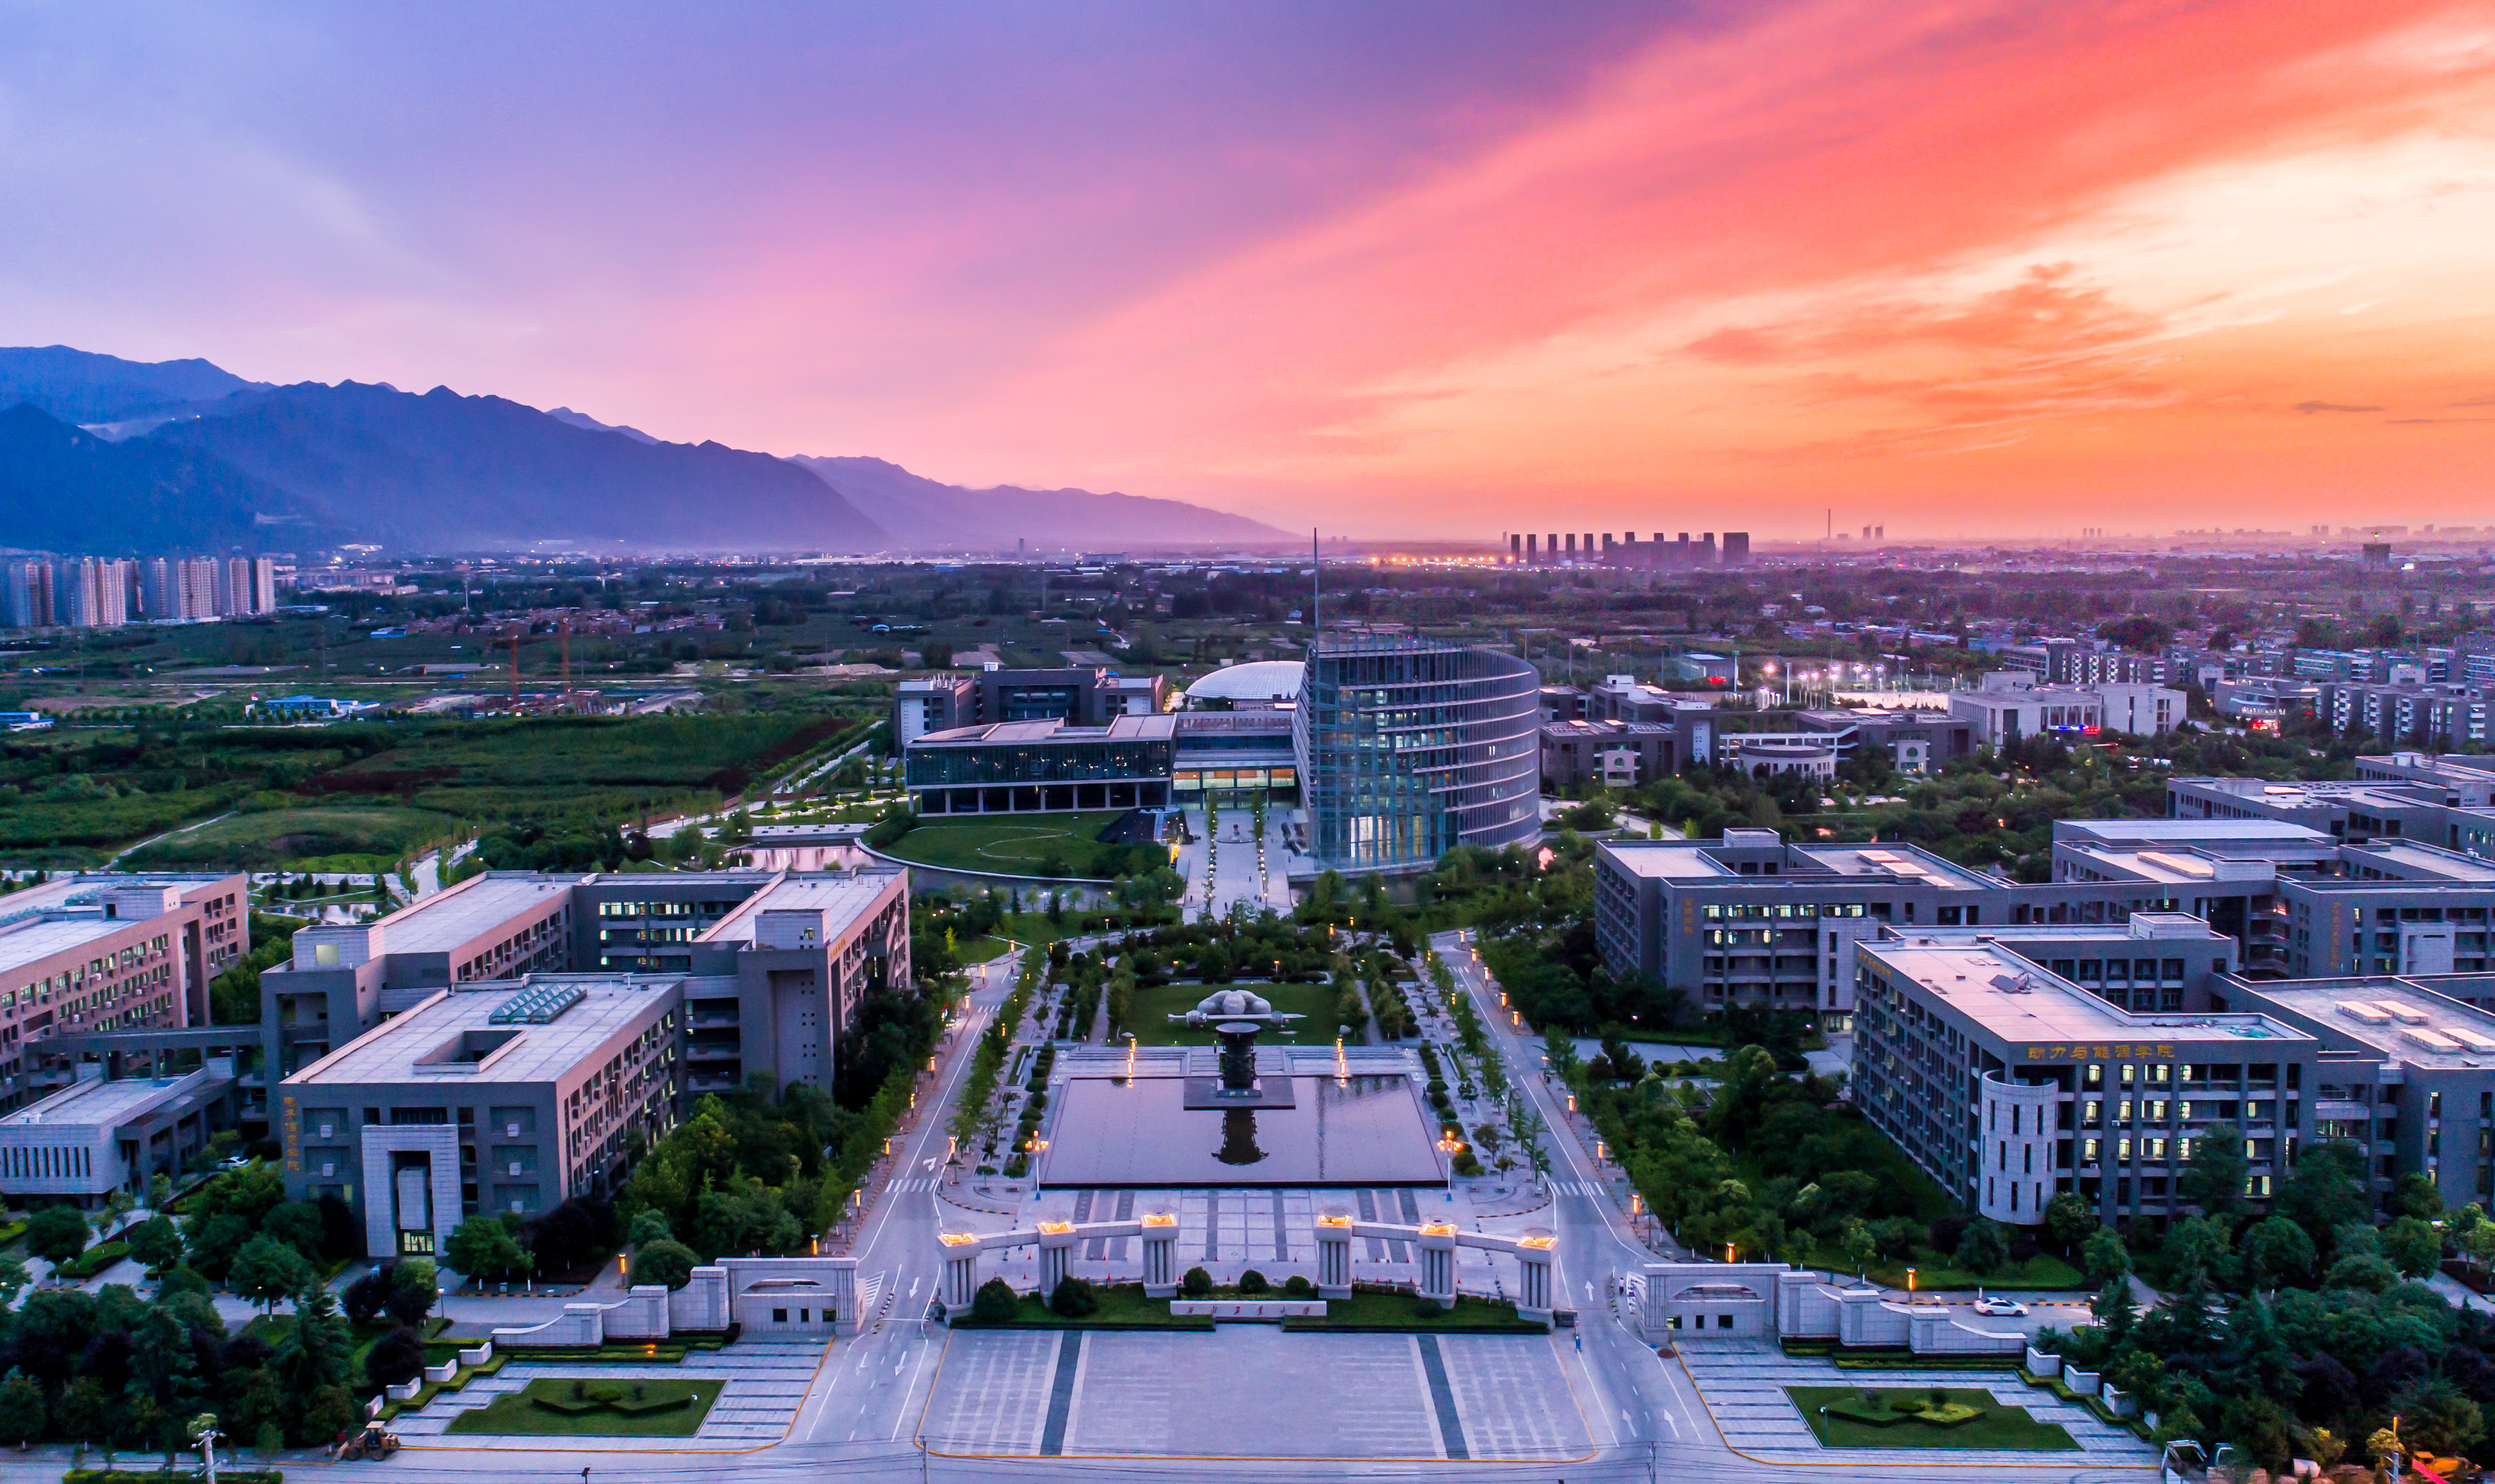
\includegraphics[width=.8\textwidth]{figures/campus.jpg}
    \caption{西工大}
\end{figure}
\lipsum[2]

% \lipsum[4-6]

\section{定理环境}
\begin{definition}
  这里是定义环境使用 `npuplain' 格式.
\end{definition}
\begin{assumption}
  这里是假设环境使用 `npuplain' 格式.
\end{assumption}
\begin{theorem}
  这里是定理环境使用 `npuplain' 格式.
\end{theorem}
\begin{lemma}
  这里是引理环境使用 `npuplain' 格式.
\end{lemma}
\begin{remark}
  这里是注环境使用 `npuplain' 格式.
\end{remark}
\begin{npu-thm}
  这里是 `' 默认的定理环境, 使用 `nputheorem' 格式.
\end{npu-thm}
% \lipsum[3]

关于养猪的文献有\parencite{Zhang2019, Zhang2019a, Zhang2019b, Zhang2019c}.

\chapter{实现}
\section{思路}
\section{代码}

\backmatter
% 以下两种参考文献格式, 根据实际宏包使用情况添加
\printbibliography             % biblatex 输出参考文件方式
% \bibliographystyle{gbt7714-2005}   % 传统输出参考文献方式
% \bibliography{ref}                 % 传统输出参考文献方式

\Appendix  % 如果有多个附录, 可重复使用该命令, 自动按字母编号.

\Thanks     % 致谢

\Work
\papersection  % 以下填写发表论文情况

\begin{npulist}
  \item {\bf Z. Yang}. NPU 硕博学位论文 \LaTeX\ 模板[D]. 2019.
\end{npulist}

\researchsection % 以下填写参加科研情况
\begin{npulist}
  \item NPU \LaTeX 模板.   编号: 000000000, 参与.
  \item NPU \LaTeX 模板.   编号: 000000001, 参与.
  \item NPU \LaTeX 模板.   编号: 000000002, 参与.
\end{npulist}

\statement
\end{document}
